\documentclass{article}


\usepackage{xcolor}
\usepackage{url}
\usepackage{blindtext}
\usepackage[english]{babel}
\usepackage{geometry}
\usepackage{nameref}
\geometry{
	a4paper,
	total={170mm,257mm},
	left=20mm,
	top=20mm,
}
\usepackage{graphicx,graphics}
\usepackage{amsmath,mathtools}
\usepackage{algpseudocode}


\renewcommand{\baselinestretch}{1.6}

%\pagecolor[HTML]{1FE9EE}%

\begin{document}
	\tableofcontents
	\listoffigures
	\listoftables
	\title{\textbf{{\Huge \textsc{Mathematics in \textcolor{red}{JEE}}}}}
	\author{\colorbox[HTML]{1FE9EE}{Ayush Gupta} \\ \emph{CSE,~IIT Dharwad} \\ \texttt{190030007@iitdh.ac.in}}
	\date{\today}
	\maketitle
	
	Joint Entrance Examination (JEE) is an engineering entrance examination conducted for admission to various engineering colleges in India. It is constituted by two different examinations - JEE Main and the JEE Advanced.
	
	\section{Major Topics in JEE \scshape{Mains}}  \label{sec: syllabus}
	
	The syllabus is includes all the topics in NCERT Maths of Class 11th and 12th. Among them, we broadly name them as follows:
	
	\begin{enumerate}
		 \item Sets and Relation
		 \item Trignometry
         \item Conic Sections
         \item Sequence and Series
         \item Quadratic Equation
         \item Complex Numbers
         \item Permutation and Combination
         \item Binomial Theorem
         \item Solution of Triangles
         \item Statistics
         \item Mathematical Reasoning
         \item Matrices and Determinants
         \item Limits and Continuity
         \item Differentiation
         \item Application of Derivative
         \item Indefinite Integrals
         \item Definite Integrsls
         \item Differential Equations
         \item Probablity
	\end{enumerate}
	
	\section{Major Topics in JEE \textsc{Advanced}}
	
	Even though JEE Advanced is significantly more difficult than JEE Mains, the syllabus is a bit less in JEE Advanced. Mathematical Reasoning, Statistics, Sets and Relations and other easy topics are not included in JEE Advanced.
	
	\section{Recommended Books}
	
	Most JEE Students follow the comprehensive books of either Cengage Publication or Arihant Publication. Here, I have listed the books of Arihant Series.
	
	\begin{description}
	
	\item [Trigonometry] for JEE by Amit M. Agarwal, is designed to bridge the gap between understanding and use of trigonometry in field of Mathematics, Science and Engineering.
        
        \begin{figure}[htp]
        	\begin{center}
        		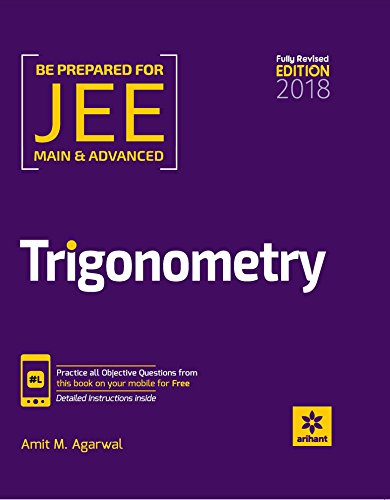
\includegraphics[width=0.15\textwidth]{Trig}
        	\end{center}
        \label{fig: Trig}
        \caption{Trignometry by Amit M Aggarwal}
        \end{figure}
    
    \item [Coordinate geometry] by Dr. SK Goyal is designed to provide a connection between algebra and geometry through graphs of lines and curves to help us locate the points in a plane.
        
        \begin{figure}[htp]
        	\begin{center}
        		\includegraphics[width=0.15\textwidth]{Coordinate}
        	\end{center}
        \label{fig: Coordinate}
        \caption{Coordinate Geometry by SK Goyal}
        \end{figure}
    
    \item [Algebra] for JEE by Dr SK Goyal, is designed to lay foundation for the most common and malleable types of mathematics used by electricians and engineers for everyday decision making or d training in science and technology.
        
        \begin{figure}[htp]
        	\begin{center}
        		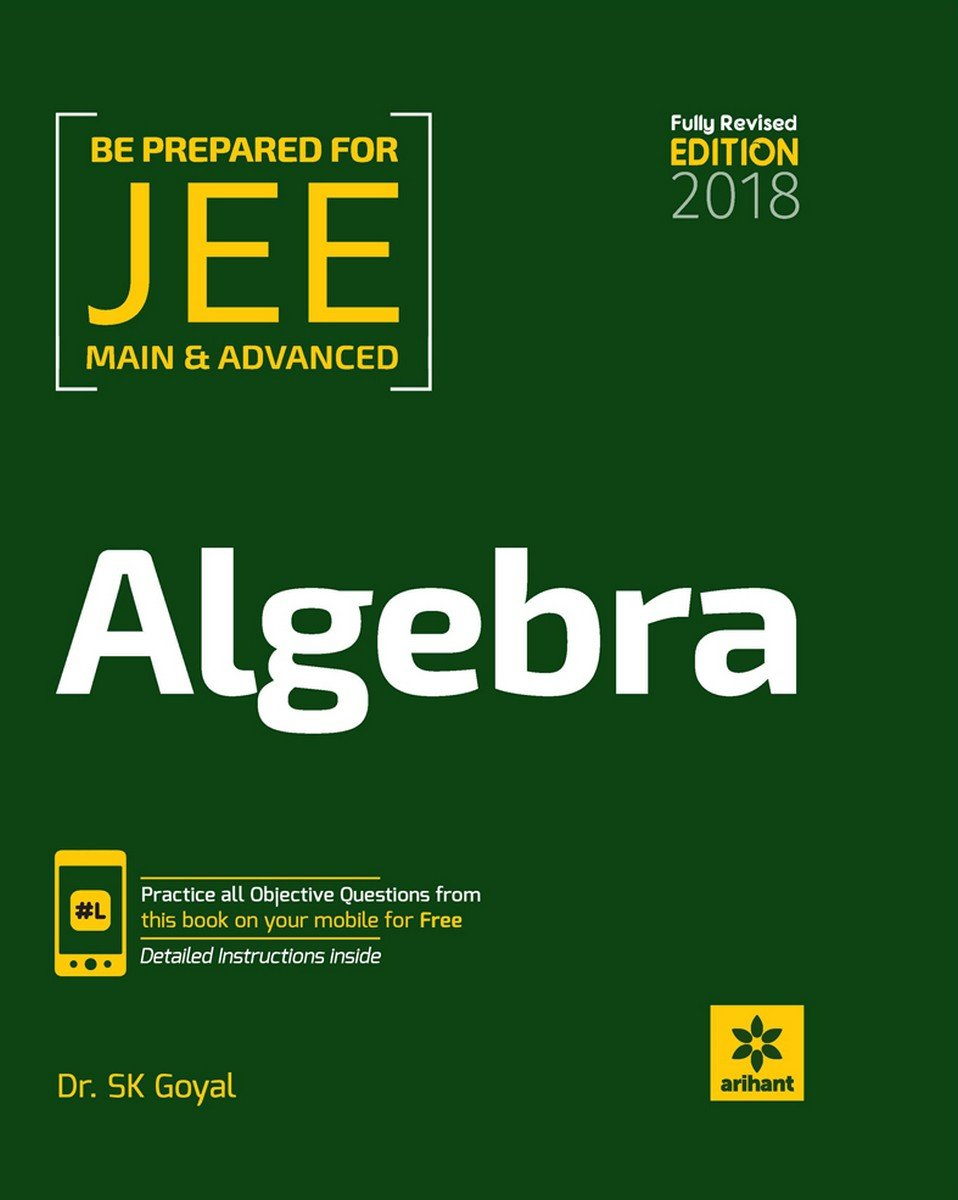
\includegraphics[width=0.15\textwidth]{Alg}
        	\end{center}
        \label{fig: Alg}
        \caption{Algebra by SK Goyal}
        \end{figure}
    
    \item [Differential Calculus] for JEE, by Amit M. Agarwal, is designed to study concepts of function derivatives, integrals, the behaviour and rate of how different quantities change on exact premise of calculus problems asked in the JEE.
        
        \begin{figure}[htp]
        	\begin{center}
        		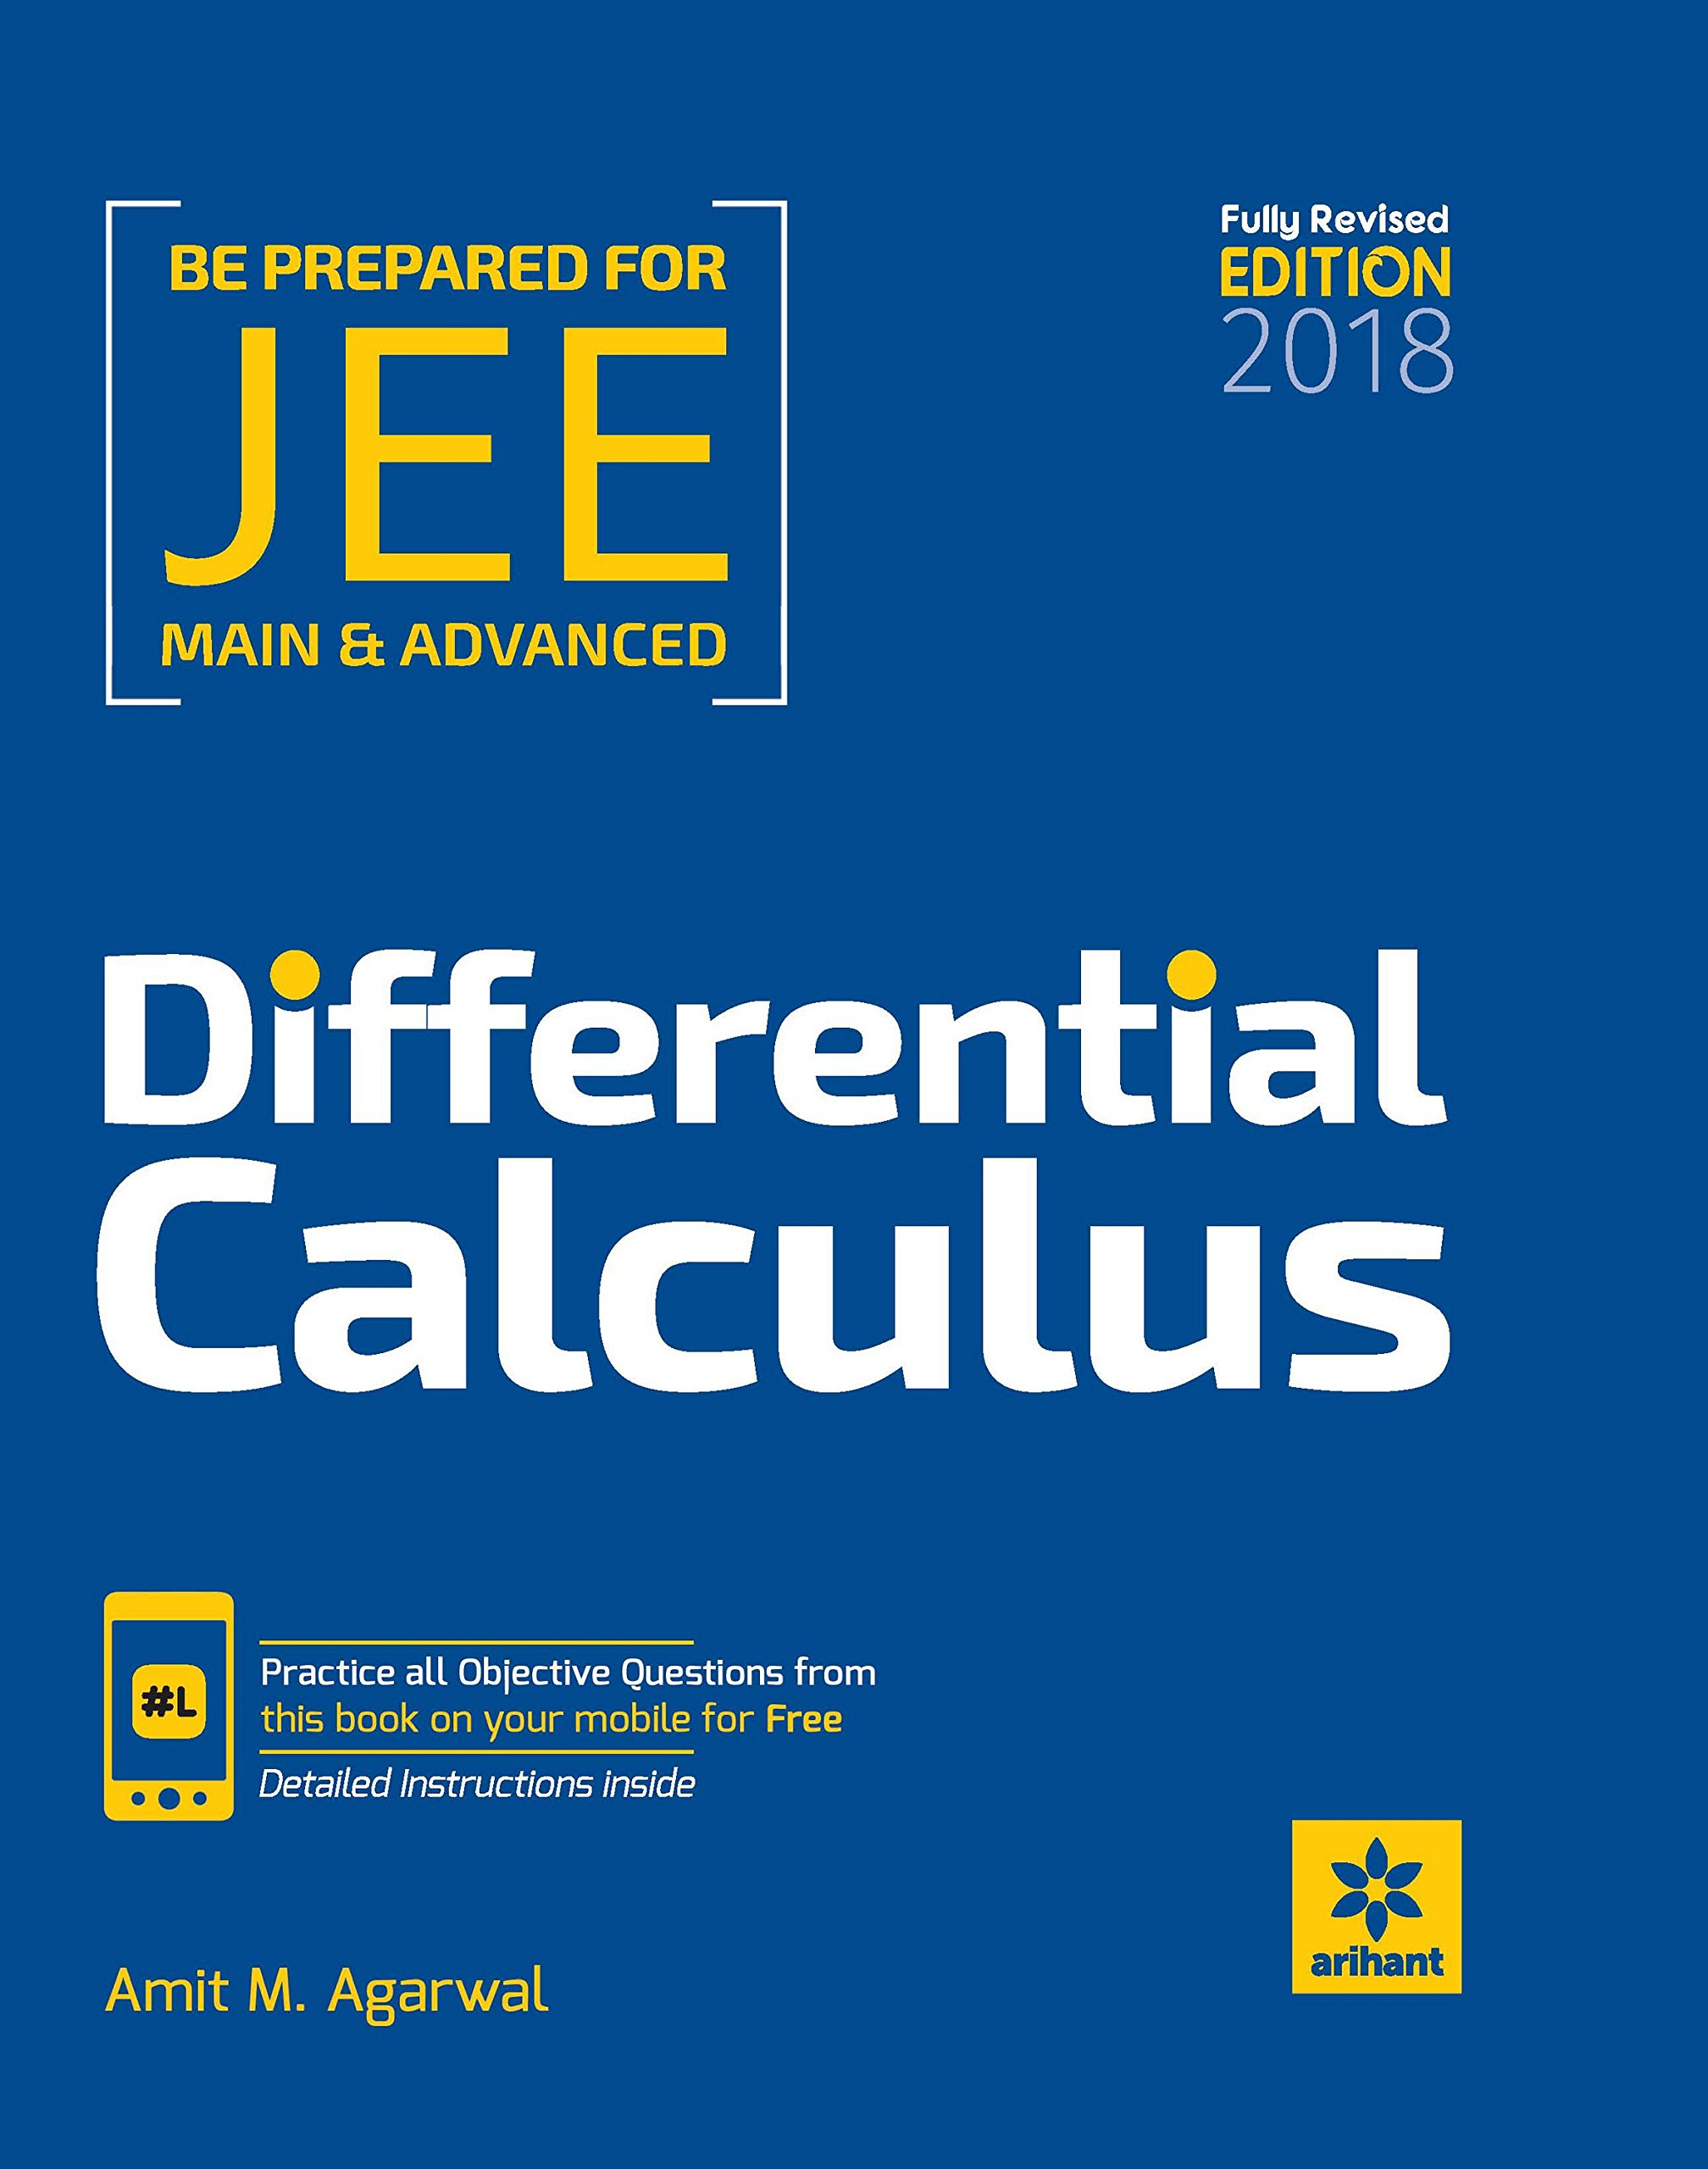
\includegraphics[width=0.15\textwidth]{Diff_Calc}
        	\end{center}
        \label{fig: Diff_Calc}
        \caption{Differential Calculus by Amit M Aggarwal}
        \end{figure}
    
    \item [Integral Calculus] by Amit M Aggarwal, is designed to take out the mystique attached with Calculus Problems breaking the problem into steps and solve them tactfully on basis of premise of calculus problems asked in the JEE Main and Advanced.
        
        \begin{figure}[htp]
        	\begin{center}
        		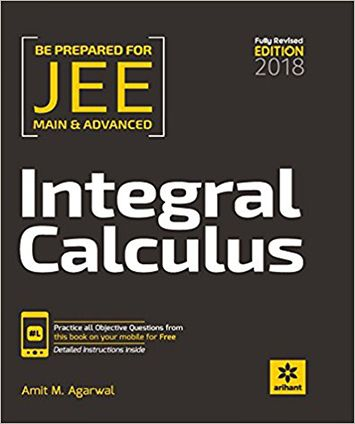
\includegraphics[width=0.15\textwidth]{Integral_Calc}
        	\end{center}
        \label{fig: Integral_Calc}
        \caption{Integral Calculus by Amit M Aggarwal}
        \end{figure}
    
    	\end{description}
    
    \section{Equations}
    
    \subsection{Rotation Matrix}
\[   \begin{bmatrix}
    	\cos \theta & \sin \theta \\
    	-\sin \theta & \cos \theta
    \end{bmatrix}   \]

For further use, check in Book~\ref{fig: Alg}
    
    \subsection{Continuity}
    
    \[ f(x) =
    \begin{cases}
    	\sin \frac{1}{x}      & \quad \text{if } x\neq0\\
    	0  & \quad \text{if } x=0
    \end{cases}
    \]
    
    Example of Discontinuous Function. For further examples, refer book~\ref{fig: Diff_Calc}
    
    \subsection{Exponential Function}
    
    \begin{align}
    	e^x & =  \sum_{n=0}^{\infty} \frac{x^n}{n!} \\
    	      & =  1 + x + \frac{x^2}{2!} + \frac{x^3}{3!} + \cdots \\
    	      & =   \frac{\mathrm d}{\mathrm d x} e^x \\
    	      & =  \int e^x {\mathrm d x}
    \end{align}

    \subsection{Heron's Formula}
    
    \begin{equation}
	\Delta = \sqrt{s\big(s-a \big)\big(s-b \big)\big(s-c \big)}
    \end{equation}

    \subsection{General Polynomial}
    
      \[f(x)= a_0 + a_1x + a_2x^2 +\dots + a_nx^n \]

    \section{Psuedocode for Quicksort Algorithm}
    \pagecolor[HTML]{ecf0cc}
    
        define Quicksort(Array,low,high)
        \begin{algorithmic}
             \If{$ low \geq high $}
                    \State $pivot \gets Partition(Array,low,high$)
                             \State Quicksort(Array,low,pivot)
                             \State Quicksort(Array,pivot,p)
                             \EndIf
        \end{algorithmic}
        define Partition(Array,low,high)
        \begin{algorithmic}
           \State $pivot \gets Array[high]$
           \State $i \gets low-1$
           \For{j in range low to high -1}
           \If { $Array[j]< pivot$ }
           \State $ i \gets i+1 $
           \State swap($Array[i],Array[j]$)
           \EndIf
           \State swap(Array[i+1], Array[high])
           \State return (i+1)
           \EndFor
        \end{algorithmic}
    
    \section{Topics Weightage in Mathematics in JEE Mains}
    
    {\centering 
    	    
        	\begin{tabular}{ | l | l | l |}
        	   \hline
        	   Name of the Topic & Expected Number of Questions & Expected Marks \\ \hline
        	   Trignometry & 02 & 08 \\ \hline
        	   Matrix and Determinant & 02 & 08 \\ \hline
        	   Probablity & 02 & 08 \\ \hline
        	   Co-ordinate Geometry & 02 & 08 \\ \hline
        	   Integral Calculus & 04 & 16 \\ \hline
        	   Differential Calculus & 07 & 28 \\ \hline
        	\end{tabular}

   }
     Refer Section~\ref{sec: syllabus} to compare. % Refering Section 1 %
    
    In \cite{ID}, Reference is present:
    
    \bibliographystyle{IEEETran}
    \bibliography{190030007_Ass1}
\end{document}